\section{Análisis y diseño}

El prototipo se desarrollará en Java, un lenguaje muy conocido. Tiene una gran cantidad de librerías y cuenta con una buena colección de herramientas para facilitar la construcción de interfaces de usuario. Además tiene entre sus grandes ventajas el ser interpretado, eliminando problemas en el desarrollo entre diferentes sistemas y arquitecturas.\\ 

Este proyecto contiene varias áreas bien diferenciadas. Para facilitar el trabajo sobre el mismo, dividiremos el proyecto en 5 áreas: Aplicación, Recuperador utilizando descriptores, Recuperador utilizando clasificaciones, Generación de descriptores y Generación de clasificaciones. Vamos a realizar un pequeño estudio de los tecnologías disponibles y el trabajo necesario para cada una de estos módulos.\\

\subsubsection{Aplicación}

En este módulo, Java pone a la disposición del desarrollador herramientas que facilitan el desarrollo de interfaces de usuario. No es necesario entonces el uso de otras librerías para el desarrollo de la interfaz. El desarrollo de éste módulo requerirá la creación de una ventana principal que permita el acceso a todas las utilidades al alcance del usuario final y las ventanas para mostrar los resultados de las distintas operaciones.\\

\subsubsection{Recuperador utilizando descriptores}

Este módulo requiere ser implementado totalmente, al no existir herramientas básicas que tengan esta funcionalidad. Se encargará de la gestión de los descriptores una vez generados. Es decir, debe realizar la tarea de creación, almacenado y carga de una base de datos de descriptores, y realizar la búsqueda y posterior recuperación de las formas en función de esto. La gestión de la base de datos se realizará de una manera simplificada, como una colección de descriptores, que se serializará para se almacenamiento y posterior recuperación. Este último detalle es evidentemente mejorable, pero para un primer prototipo es suficiente.\\

\subsubsection{Recuperador utilizando clasificaciones}

Igual que en el módulo anterior, requiere ser implementado totalmente. De manera similar, también requiere realizar la tarea de la gestión de una base de datos de clasificaciones y la búsqueda. En este caso además, se requiere el almacenamiento de los datos de los resultados del clasificador, es decir, para cada valor de la predicción del clasificador poder decir el concepto asociado así como sus predecesores en la arquitectura jerárquica de WordNet.\\

\subsubsection{Generación de descriptores}

Se utilizará una librería, llamada Java Fuzzy Imaging (JFI). En concreto, se utilizarán los paquetes relacionados con formas, desarrollado conjuntamente con el director de este proyecto, Jesús Chamorro Martínez. La labor de este módulo es la creación de los descriptores utilizados en el projecto, la curvatura y la curvacidad.\\
  
\subsubsection{Generación de clasificadores}

Se ha comentado en el capítulo \ref{ch2} que se ha usado la librería Caffe para el entrenamiento del modelo. Esta librería es muy sencilla de usar, pero no tiene interfaz para el lenguaje Java. El problema aquí es que el único paquete disponible en el lenguaje Java que contiene el tipo de redes que se necesita aplicar a este problema es la librería DeepLearning4J, que es de pago. Dado que el resto de librerías de este ámbito (Torch, TensorFlow,...) tampoco tienen una API para Java, se eligió Caffe por su facilidad de uso y buen rendimiento.\\

\subsection{Casos de uso}

\subsubsection{Abrir imagen}

\begin{itemize}
\item \textbf{Nombre: }Abrir imagen.
\item \textbf{Descripción: }El usuario indica que quiere abrir una imagen y selecciona la imagen en un menú. El sistema carga dicha imagen y se la muestra al usuario.
\item \textbf{Actor: }Usuario.
\item \textbf{Precondición: } 
\item \textbf{Flujo normal: }
\begin{enumerate}
\item El usuario acciona el botón ``Abrir imagen''.
\item El sistema muestra un navegador para que el usuario seleccione la imagen.
\item El usuario selecciona una imagen.
\item El sistema carga la imagen.
\item Se muestra la imagen al usuario.
\end{enumerate}
\item \textbf{Flujo alternativo:}
\begin{itemize}
\item (3.1) El usuario cancela la selección y se termina el proceso.
\end{itemize}
\item \textbf{Postcondición: }Se crea una ventana con la imagen.
\end{itemize}

\subsubsection{Abrir base de datos}

\begin{itemize}
\item \textbf{Nombre: }Abrir base de datos.
\item \textbf{Descripción: }El usuario indica que quiere abrir una base de datos y la selecciona en un menú. El sistema carga dicha base de datos en el sistema, e indica al usuario la base abierta y su tipo.
\item \textbf{Actor: }Usuario.
\item \textbf{Precondición: }
\item \textbf{Flujo normal: }
\begin{enumerate}
\item El usuario acciona el botón ``Abrir base de datos.''
\item El sistema muestra un navegador para que el usuario seleccione la base de datos.
\item El usuario selecciona una base de datos.
\item El sistema determina el tipo de base de datos.
\item El sistema carga la base de datos según su tipo.
\item Se muestra al usuario la base de datos abierta en un mensaje del interfaz.
\end{enumerate}
\item \textbf{Flujo alternativo:}
\begin{itemize}
\item (3.1) El usuario cancela la selección y se termina el proceso.
\item (4.1) La base de datos no es correcta, se cancela la operación.
\end{itemize}
\item \textbf{Postcondición: } El sistema tiene abierta para consultas la base de datos indicada. Mediante el interfaz se muestran tanto el nombre como el tipo de la base seleccionada.
\end{itemize}

\subsubsection{Clasificar imagen seleccionada}

\begin{itemize}
\item \textbf{Nombre: }Clasificar imagen seleccionada.
\item \textbf{Descripción: } El usuario indica que quiere clasificar la imagen seleccionada, y el sistema muestra al usuario el resultado de la clasificación.
\item \textbf{Actor: }Usuario.
\item \textbf{Precondición: }El usuario tiene una imagen activa.
\item \textbf{Flujo normal: }
\begin{enumerate}
\item El usuario acciona el botón ``Clasificar imagen''.
\item El sistema recupera la información de la imagen seleccionada.
\item Se clasifica la imagen.
\item Se muestra al usuario el resultado.
\end{enumerate}
\item \textbf{Flujo alternativo:}
\begin{itemize}
\item (1.1) El usuario no tiene una imagen activa, el proceso termina.
\end{itemize}
\item \textbf{Postcondición: }Se crea una ventana de clasificación con los resultados.
\end{itemize}

\subsubsection{Seleccionar tipo de descriptor utilizado}

\begin{itemize}
\item \textbf{Nombre: }Seleccionar tipo de descriptor utilizado.
\item \textbf{Descripción: }El usuario elige el descriptor a utilizar y el sistema almacena esa preferencia.
\item \textbf{Actor: }Usuario.
\item \textbf{Precondición: }
\item \textbf{Flujo normal: }
\begin{enumerate}
\item El usuario selecciona ``descriptor utilizado''.
\item El sistema muestra las distintas opciones.
\item El usuario selecciona una de las opciones.
\end{enumerate}
\item \textbf{Flujo alternativo:}
\item \textbf{Postcondición: }El sistema empieza a utilizar el descriptor indicado.
\end{itemize}

\subsubsection{Calcular descriptor de la imagen seleccionada}

\begin{itemize}
\item \textbf{Nombre: }Calcular descriptor de la imagen seleccionada.
\item \textbf{Descripción: }El usuario indica que quiere calcular el descriptor de una forma seleccionada, y el sistema muestra al usuario el resultado del cálculo del descriptor.
\item \textbf{Actor: }Usuario.
\item \textbf{Precondición: }El usuario tiene una forma activa.
\item \textbf{Flujo normal: }
\begin{enumerate}
\item El usuario acciona el botón ``Calcular descriptor de forma''.
\item El sistema recupera la información de la forma seleccionada.
\item Se calcula el descriptor de la forma en base a la medida activa.
\item Se muestra al usuario el resultado.
\end{enumerate}
\item \textbf{Flujo alternativo:}
\begin{itemize}
\item (1.1) El usuario no tiene una forma activa, el proceso termina.
\end{itemize}
\item \textbf{Postcondición: }Se crea una ventana de descriptor con los resultados.
\end{itemize}

\subsubsection{Buscar con un descriptor}

\begin{itemize}
\item \textbf{Nombre: }Buscar con un descriptor.
\item \textbf{Descripción: } El usuario indica que quiere buscar en base al descriptor seleccionado en la base de datos, y el sistema la muestra de manera ordenada toda la base de datos según su búsqueda.
\item \textbf{Actor: }Usuario.
\item \textbf{Precondición: }Hay una ventana de descriptor activa y una base de datos de descriptores activa.
\item \textbf{Flujo normal: }
\begin{itemize}
\item El usuario acciona el botón ``Búsqueda por descriptor''.
\item El sistema ordena las formas de la base de datos activa según su proximidad al descriptor consultado.
\item El sistema muestra los formas de manera ordenada.
\end{itemize}
\item \textbf{Flujo alternativo:}
\item \textbf{Postcondición: }Se crea una ventana con los resultados de la búsqueda.
\end{itemize}

\subsubsection{Buscar por un concepto}

\begin{itemize}
\item \textbf{Nombre: }Buscar por un concepto.
\item \textbf{Descripción: }El usuario indica el concepto a buscar en la base de datos y el sistema muestra ordenadamente las imágenes de la base de datos según su cumplimiento del concepto.
\item \textbf{Actor: }Usuario.
\item \textbf{Precondición: }El sistema tiene una base de datos de clasificaciones activa.
\item \textbf{Flujo normal: }
\begin{itemize}
\item El usuario escribe el concepto y acciona el botón ``Búsqueda por concepto''.
\item El sistema ordena las imágenes de la base de datos activa según su grado de cumplimiento del concepto indicado.
\item El sistema muestra los imágenes de manera ordenada.
\end{itemize}
\item \textbf{Flujo alternativo:}
\item \textbf{Postcondición: }Se crea una ventana con los resultados de la búsqueda.
\end{itemize}

\subsubsection{Crear base de datos}

\begin{itemize}
\item \textbf{Nombre: }Crear base de datos.
\item \textbf{Descripción: }El administrador indica el tipo de base de datos a generar, la carpeta a clasificar y donde guardar la base de datos, y el sistema realiza la acción. Proceso realizado fuera de la aplicación.
\item \textbf{Actor: }Administrador del sistema.
\item \textbf{Precondición: }
\item \textbf{Flujo normal: }
\begin{itemize}
\item El administrador indica: tipo de base de datos, carpeta de entrada y dirección donde guardar la base de datos.
\item El sistema almacena la nueva base de datos.
\end{itemize}
\item \textbf{Flujo alternativo:}
\item \textbf{Postcondición: } Se genera y almacena la nueva base de datos.
\end{itemize}

\subsection{Diagrama de casos de uso}
\begin{figure}[H]
\begin{center}

\includegraphics[width=0.9\textwidth]{img/diagramadecasosdeuso.pdf}
\end{center}

\caption{Diagrama de casos de uso.}
\label{casouso}
\end{figure}

En la figura \ref{casouso} encontramos el diagrama de casos de uso. Este sirve de pequeño resumen de los casos de uso del sistema. Podemos ver claramente las acciones que se deben implementar en la aplicación, todas en las que participa el usuario. Además destacamos la existencia de un caso de uso del administrador del sistema, la creación de base de datos, pues este puede ser un proceso muy pesado para la ejecución durante el uso del usuario, provocando bloqueos muy largos de la aplicación. Por tanto, esa tarea se realizará off-line por el administrador, quedando fuera de la aplicación.\\

\subsection{Diagrama de estados}

Vamos a realizar los diagramas de estado, pero solo de los procesos más significativos. Esto se hace dado que hay varios procesos muy similares, como abrir imagen y abrir base de datos. Por tanto se han elegido los más significativos para evitar caer en repeticiones innecesarias.

\subsubsection{Abrir base de datos}
\begin{figure}[H]
\begin{center}

\includegraphics[width=0.7\textwidth]{img/abrirdb.pdf}
\end{center}

\caption{Diagrama de estados de ``Abrir base de datos''.}
\label{abrirdb}
\end{figure}

\subsubsection{Clasificar imagen seleccionada}
\begin{figure}[H]
\begin{center}

\includegraphics[width=0.6\textwidth]{img/classimg.pdf}
\end{center}

\caption{Diagrama de estados de ``Clasificar imagen seleccionada''.}
\label{classimg}
\end{figure}

\subsubsection{Buscar con un concepto}
\begin{figure}[H]
\begin{center}

\includegraphics[width=0.6\textwidth]{img/searchc.pdf}
\end{center}

\caption{Diagrama de estados de ``Buscar con un concepto''.}
\label{searchc}
\end{figure}

\subsection{Diagrama de clases}

Vamos a mostrar los diagramas de clases de los módulos principales de la aplicación, los módulos de búsqueda, obviando el del módulo de la aplicación, que se limita a una clase ``MainWindow'' que tiene todos los métodos asociados a los distintos botones, y un conjunto de clases asociadas, una por cada ventana interna de la aplicación.

\begin{figure}[H]
\begin{center}

\includegraphics[width=1\textwidth]{img/clases-desc.pdf}
\end{center}

\caption{Diagrama de clases del módulo ``Buscar con descriptores''.}
\end{figure}

Podemos apreciar una estructura muy simple. Tenemos una clase de tipo ``Factory'' que crea las instancias tanto de una base de datos de descriptores como de descriptores de contornos. Realiza esta tarea llamando a la librería JFI. La clase ``FeatureDB'' gestiona una colección de descriptores, permitiéndonos buscar por ellos. La clase ``ContourFeature'' se encarga de almacenar y modificar los valores de la característica.\\

\begin{figure}[H]
\begin{center}

\includegraphics[width=1\textwidth]{img/clases-class.pdf}
\end{center}

\caption{Diagrama de clases del módulo ``Buscar con clasificación''.}
\end{figure}

Este módulo sigue una estructura similar al anterior, con dos añadidos. Por un lado, la clasificación de una imagen no será una lista de valores, si no un árbol, por lo que es necesario crear una clase que represente un nodo del mismo. Por otro lado, tenemos que ser capaces de traducir los indices de respuesta del clasificador por palabras reales a las que encontrar significado, por ello introducimos la clase ``SynsetDictionary'', para encapsular estas funcionalidades.
\subsection{Explicación de los tipos de datos y algoritmos fundamentales}

\subsubsection{Búsqueda por descriptor}

La búsqueda por descriptor sigue el siguiente algoritmo, siendo ``consulta'' el descriptor consultado:
\begin{itemize}
\item Para cada descriptor de la base de datos:
\begin{itemize}
\item Calcular la distancia euclídea entre el descriptor y la consulta.
\item Añadir al array de salida el resultado y la dirección de la imagen asociada al descriptor.
\end{itemize}
\item Se ordena según la distancia, a más pequeña mejor.
\end{itemize}

Pero para poder comparar dos descriptores, tenemos que realizar algunas modificaciones en los mismos, pues dos formas pueden ser perfectamente iguales, pero tener descriptores distintos dependiendo del punto donde se empezaron a calcular. También pueden influir factores de escala, que cambien la escala del resultado. Por tanto, para evitar esta problemática, a cada descriptor se le aplica siempre los dos siguientes pasos:
\begin{itemize}
\item Normalizar el descriptor al intervalo [0,1].
\item Colocar como primer elemento el mayor.
\end{itemize}

Así podemos ya comparar de manera directa mediante el uso de una distancia, en este caso la euclídea.

\subsubsection{Tipo de dato de clasificación de una imagen}

Los términos aprendidos, pertenecen a una estructura jerárquica. En la figura \ref{arbol} podemos ver un caso reducido de este suceso. Si sólo mantenemos los valores aprendidos (fila inferior), podremos buscar por tipos concretos de animales, pero no por conceptos más generales como ``perro'' o ``animal''.\\

\begin{figure}
\begin{center}

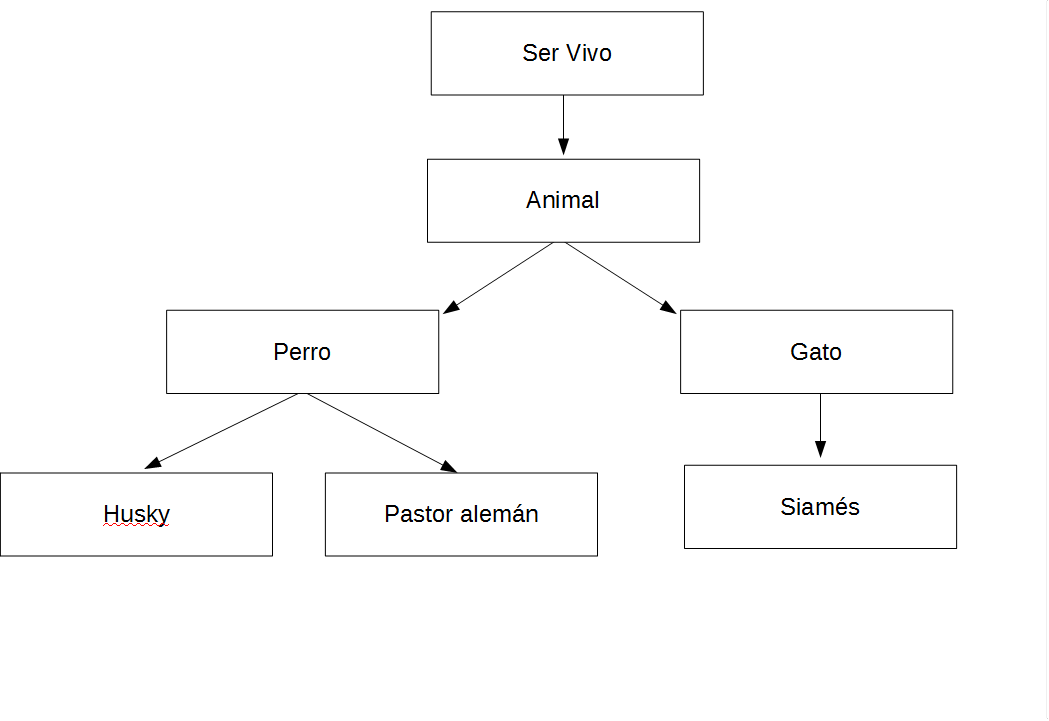
\includegraphics[width=0.5\textwidth]{img/arbol.PNG}
\end{center}

\caption{Ejemplo reducido de la estructura de clasificación de una imagen.}
\label{arbol}
\end{figure}


Por tanto, una clasificación de una imagen será un árbol. La valoración de un nodo padre será la del mejor de sus nodos hijos. Se hace necesario entonces, para poder conocer el valor de un concepto concreto dentro de esta estructura, el poder buscar dentro del árbol.

\subsubsection{Búsqueda por concepto}

Para buscar en el árbol un concepto, vamos a hacerlo en profundidad, el objetivo es tratar de encontrar las respuestas más genéricas posibles. Aún así, podríamos encontrarnos categorías con conceptos muy similares. Por tanto, seguiremos la búsqueda hasta que estemos seguros que no vamos a encontrar un concepto que lo represente mejor.\\

El algoritmo sería así:
\begin{itemize}
\item Se inserta en la cola de búsqueda al nodo raíz.
\item Para cada elemento de la cola:
\begin{itemize}
\item Obtener su concepto asociado.
\item Si contiene el concepto a buscar, y supera al mejor encontrado, es el nuevo mejor concepto para la búsqueda.
\item Si la búsqueda tiene más creencia que 0.5, hemos terminado la búsqueda.
\item Si no se ha terminado la búsqueda, se incluyen sus hijos en la cola y se sigue buscando.
\end{itemize}
\item Se devuelve el mejor valor de creencia encontrado.
\end{itemize}